\documentclass{jsarticle}
\usepackage{amsmath,amssymb}
\usepackage{enumerate}
\usepackage[dvipdfmx]{graphicx}
\usepackage[dvipdfmx]{color}
\usepackage{here}
\usepackage{breqn}
\usepackage{amsthm}
\theoremstyle{definition}
\usepackage{bm}
\newtheorem{Ex}{問題}
%\newtheorem*{Ex*}{演習問題}
\newtheoremstyle{mystyle}%   % スタイル名
    {}%                      % 上部スペース
    {}%                      % 下部スペース
    {\normalfont}%           % 本文フォント
    {}%                      % インデント量
    {\bf}%                   % 見出しフォント
    {}%                      % 見出し後の句読点, '.'
    { }%                     % 見出し後のスペース, ' ' or \newline
    {\underline{\thmname{#1}\thmnumber{#2}\thmnote{(#3)}}}%
                             % 見出しの書式 (can be left empty, meaning `normal')
\theoremstyle{mystyle} % スタイルの適用
\newtheorem*{Def}{Def}
\newtheorem*{theo}{Theorem}
\newtheorem*{lem}{Lemma}
\newtheorem{ex}{example}
\newtheorem*{col}{Corollary}
\renewcommand{\footnotesize}{\normalsize}
\usepackage{latexsym}
\usepackage{color}
\usepackage{emathEy}
\usepackage{listings,plistings}
\def\qed{\hfill$\Box$}
\lstset{
language={Python},
backgroundcolor={\color[gray]{.85}},
basicstyle={\footnotesize},
identifierstyle={\footnotesize},
commentstyle={\footnotesize\ttfamily \color[rgb]{0,0.5,0}},
keywordstyle={\footnotesize\bfseries \color[rgb]{1,0,0}},
ndkeywordstyle={\footnotesize},
stringstyle={\footnotesize\ttfamily \color[rgb]{0,0,1}},
frame={tb},
breaklines=true,
columns=[l]{fullflexible},
numbers=left,
xrightmargin=0zw,
xleftmargin=3zw,
numberstyle={\scriptsize},
stepnumber=1,
numbersep=1zw,
morecomment=[l]{//}
}

\begin{document}
\large
\begin{Ex}
\begin{enumerate}[(a)]
  \item $f(x,y)=\sqrt{x^2+y^2}$の$(x,y)\neq (0,0)$における偏微分をそれぞれ求めると
  \begin{align*}
    \frac{\partial f}{\partial x}(x,y)&=\frac{x}{\sqrt{x^2+y^2}}\\
    \frac{\partial f}{\partial y}(x,y)&=\frac{y}{\sqrt{x^2+y^2}}
  \end{align*}
となる.\\

\item $p\geq 2$に対し,$\beta=(\beta_1,\cdots,\beta_p)\neq 0$における$\|\beta\|_2$の$\beta_i(1\leq i\leq p)$における偏微分は
\begin{align*}
  \frac{\partial \|\beta\|}{\partial \beta_i}&=\frac{\beta_i}{\|\beta\|_2}
\end{align*}
となることより,$\|\beta\|_2$の$\beta\neq 0$における偏微分は
$$\frac{\partial \|\beta\|}{\partial \beta}=\frac{\beta}{\|\beta\|_2}$$
となる.\\

\item $f(x,y)$の$(x_0,y_0)=(0,0)$における劣微分を求める.$(u,v)\in\mathbb{R}^2$が劣微分の要素であったとする.すなわち,任意の$(x,y)\in \mathbb{R}^2$に対して
\begin{align}
  \label{retsu}
  f(x,y)\geq ux+vy
\end{align}
を満たしているとする.ここで,$r,s>0,0\leq \theta,\phi< 2\pi$を用いて
\begin{align*}
  x&=r\cos\theta,\quad y =r\sin\theta\\
  u&=s\cos\phi,\quad v = s\sin\phi
\end{align*}
と極座標変換を行うと,(\ref{retsu})式は
\begin{align*}
  r&\geq sr\cos\theta\cos\phi+sr\sin\theta\sin\phi\\
&=rs\cos(\theta-\phi)\\
\therefore 1&\geq s\cos(\theta-\phi)
\end{align*}
とかくことができる.上式が成立することの必要十分条件は$s\geq 1$であることなので,求める劣微分は
$$\{(u,v)\in\mathbb{R}^2\mid u^2+v^2\leq 1\}$$
となる.\qed
\end{enumerate}
\end{Ex}
%%%%%%%%%%%%%%%%%%%%%%%%%%%%%%
\begin{Ex}
$g(z)=\frac{1}{2}(y-Xz)^2$のヘッセ行列$\nabla^2 g(x)$を求めると
\begin{align*}
  \frac{\partial g}{\partial z}(z)&=-X^T(y-Xz)\\
  \frac{\partial g}{\partial z}(z)&=X^TX
\end{align*}
となることがわかる.ここで$X^TX$は非負定値行列であることより,$X^TX$の二次形式の最大値は$X^TX$の最大固有値$\lambda_{max}$に一致するので,任意の$x,y,z\in \mathbb{R}^p$に対して
\begin{align*}
  (x-y)^T \nabla^2g(z)(x-y)&=(x-y)^tX^TX(x-y)\\
  &\leq \lambda_{max}\|x-y\|_2^2
\end{align*}
が成立することがわかる.上式で$\lambda_{max}=L$とすれば求めたい不等式が得られる.\qed\\
\end{Ex}
%%%%%%%%%%%%%%%%%%%%%%%%%%%%%
\begin{Ex}
  空欄を埋めたプログラムは下の通り.
  \begin{lstlisting}[basicstyle = \ttfamily\footnotesize, frame = single]
def group_lasso(z, y, lam=0):
    J = len(z)
    theta = []
    for i in range(J):
        theta.append(np.zeros(z[i].shape[1]))
    for m in range(10):
        for j in range(J):
            r = copy.copy(y)
            for k in range(J):
                if k != j:
                    r = r - z[k] @ theta[k]
            theta[j] = gr(z[j], r, lam)
    return theta
  \end{lstlisting}

  \begin{lstlisting}[basicstyle = \ttfamily\footnotesize, frame = single]
n = 100
J = 2
u = randn(n)
v = u + randn(n)
s = 0.1 * randn(n)
t = 0.1 * s + randn(n)
y = u + v + s + t + randn(n)
z = []
z = np.array([np.array([u, v]).T, np.array([s, t]).T])
lambda_seq = np.arange(0, 500, 10)
m = len(lambda_seq)
beta = np.zeros((m, 4))
for i in range(m):
    est = group_lasso(z, y, lambda_seq[i])
    beta[i, :] = np.array([est[0][0], est[0][1], est[1][0], est[1][1]])
plt.xlim(0, 500)
plt.ylim(np.min(beta), np.max(beta))
plt.xlabel(r"$\lambda$")
plt.ylabel("係数の値")
labels = ["グループ1", "グループ1", "グループ2", "グループ2"]
cols = ["red", "blue"]
lins = ["solid", "dashed"]
for i in range(4):
    plt.plot(lambda_seq, beta[:, i], color=cols[i//2],
             linestyle=lins[i % 2], label="{}".format(labels[i]))
plt.legend(loc="upper right")
plt.axvline(0, color="black")
plt.show()
    \end{lstlisting}
上記の実行結果は以下の様になる.
\begin{figure}[H]
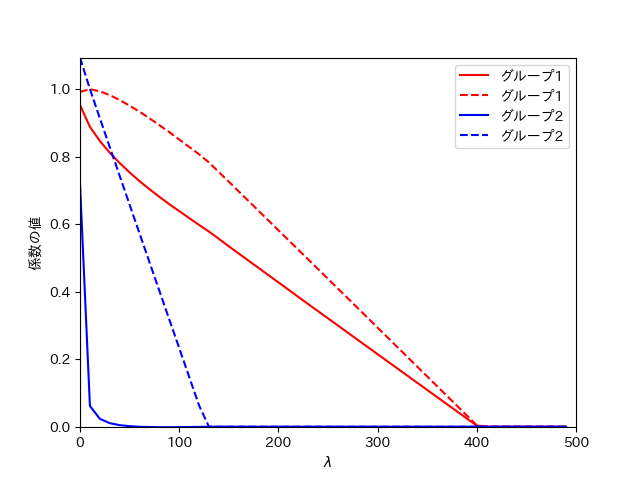
\includegraphics[width=10cm]{gr.png}
\end{figure}
\end{Ex}
%%%%%%%%%%%%%%%%%%%%%%%%%%%%%%%%%%%%%
\begin{Ex}
目的関数$L$は
$$L=\frac{1}{2}\|y-X\sum_{k=1}^K\theta_k\|_2^2 +\lambda\sum_{k=1}^K\|\theta_k\|_2$$
である.ただし
\begin{align*}
  \theta_1=\left(\begin{array}{c}
    \beta_1\\
    \beta_2\\
    \beta_{3,1}\\
    0\\
    0
  \end{array}\right),\quad \theta_2=\left(\begin{array}{c}
    0\\
    0\\
    \beta_{3,2}\\
    \beta_4\\
    \beta_5
  \end{array}\right)\quad (\beta_3=\beta_{3,1}+\beta_{3,2})
\end{align*}
として,$\beta=\theta_1+\theta_2$とした.ここで,$X$の最初の3列を$X_1\in\mathbb{R}^{N\times 3}$,最後の3列を$X_2\in \mathbb{R}^{N\times 3}$と書き,$\theta_1,\theta_2$の非ゼロ成分$\gamma_1,\gamma_2$で$L$に関して劣微分をとると
\begin{align*}
  \frac{\partial L}{\partial \gamma_1}&=-X_1^T(y-X_1\gamma_1)+\lambda\partial\|\gamma_1\|_2\\
  \frac{\partial L}{\partial \gamma_2}&=-X_2^T(y-X_2\gamma_2)+\lambda\partial\|\gamma_2\|_2\\
\end{align*}
と書くことができる.したがって$L$を$\beta$で微分して$0$とおく式は
\begin{align*}
  -X_1^T(y-X\theta_1)+\lambda\partial\|\gamma_1\|_2&=0\\
  -X_2^T(y-X\theta_2)+\lambda\partial\|\gamma_2\|_2&=0
\end{align*}
となるので,上式において$\theta_j=0(j=1,2)$とおくと
\begin{align*}
  X_j^Ty &=\lambda\partial\|\gamma_j\|_2\Leftrightarrow \|X_i^Ty\|_2\leq \lambda\quad(i=1,2)
\end{align*}
となる.最右辺が求める条件である.\qed\\
\end{Ex}
%%%%%%%%%%%%%%%%%%%%%%%%%%%%%%%%%%%%%%%%%%%
\begin{Ex}
  空欄を埋めたプログラムは下の通り
  \begin{lstlisting}[basicstyle = \ttfamily\footnotesize, frame = single]
  def gr_multi_lasso(X, y, lam):
    n = X.shape[0]
    p = X.shape[1]
    K = len(np.unique(y))
    beta = np.ones((p, K))
    Y = np.zeros((n, K))
    for i in range(n):
        Y[i, y[i]] = 1
    eps = 1
    while eps > 0.001:
        gamma = copy.copy(beta)
        eta = X @ beta
        P = np.exp(eta)
        for i in range(n):
            P[i, ] = P[i, ] / np.sum(P[i, ])
        t = 2 * np.max(P*(1-P))
        R = (Y-P) / t
        for j in range(p):
            r = R + X[:, j].reshape(n, 1) @ beta[j, :].reshape(1, K)
            M = X[:, j] @ r
            beta[j, :] = (max(1 - lam / t / np.sqrt(np.sum(M*M)), 0)
                          / np.sum(X[:, j]*X[:, j]) * M)
            R = r - X[:, j].reshape(n, 1) @ beta[j, :].reshape(1, K)
        eps = np.linalg.norm(beta - gamma)
    return beta
\end{lstlisting}


\begin{lstlisting}[basicstyle = \ttfamily\footnotesize, frame = single]
  iris = load_iris()
  X = np.array(iris["data"])
  y = np.array(iris["target"])
  
  lambda_seq = np.arange(10, 151, 10)
  m = len(lambda_seq)
  p = X.shape[1]
  K = 3
  alpha = np.zeros((m, p, K))
  for i in range(m):
      res = gr_multi_lasso(X, y, lambda_seq[i])
      alpha[i, :, :] = res
  plt.xlim(0, 150)
  plt.ylim(np.min(alpha), np.max(alpha))
  plt.xlabel(r"$\lambda$")
  plt.ylabel("係数の値")
  handles = []
  labels = ["がく片の長さ", "がく片の幅", "花びらの長さ", "花びらの幅"]
  cols = ["red", "green", "blue", "cyan"]
  for i in range(4):
      for k in range(K):
          line, = plt.plot(lambda_seq, alpha[:, i, k], color=cols[i],
                           label="{}".format(labels[i]))
      handles.append(line)
  plt.legend(handles, labels, loc="upper right")
\end{lstlisting}
また実行結果は下の通り
\begin{figure}[H]
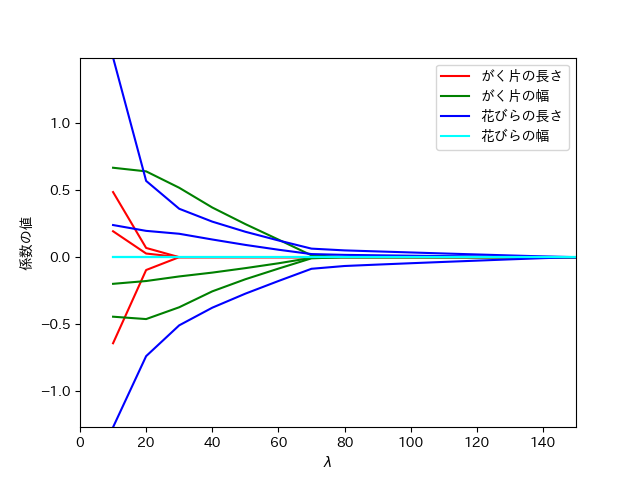
\includegraphics[width=10cm]{iris.png}
 \end{figure}
\end{Ex}


\end{document}
